\documentclass[final]{beamer}

\usepackage[scale=1.24]{beamerposter} % Use the beamerposter package for laying out the poster

\usepackage{tikz} % Add this package for overlay

\usetheme{confposter} % Use the confposter theme supplied with this template

\setbeamercolor{block title}{fg=ngreen,bg=white} % Colors of the block titles
\setbeamercolor{block body}{fg=black,bg=white} % Colors of the body of blocks
\setbeamercolor{block alerted title}{fg=white,bg=dblue!70} % Colors of the highlighted block titles
\setbeamercolor{block alerted body}{fg=black,bg=dblue!10} % Colors of the body of highlighted blocks
% Many more colors are available for use in beamerthemeconfposter.sty

% Define the column widths and overall poster size
% To set effective sepwid, onecolwid and twocolwid values, first choose how many columns you want and how much separation you want between columns
% In this template, the separation width chosen is 0.024 of the paper width and a 4-column layout
% onecolwid should therefore be (1-(# of columns+1)*sepwid)/# of columns e.g. (1-(4+1)*0.024)/4 = 0.22
% Set twocolwid to be (2*onecolwid)+sepwid = 0.464
% Set threecolwid to be (3*onecolwid)+2*sepwid = 0.708

\newlength{\sepwid}
\newlength{\onecolwid}
\newlength{\twocolwid}
\newlength{\threecolwid}
\setlength{\paperwidth}{48in} % A0 width: 46.8in
\setlength{\paperheight}{36in} % A0 height: 33.1in
\setlength{\sepwid}{0.024\paperwidth} % Separation width (white space) between columns
\setlength{\onecolwid}{0.22\paperwidth} % Width of one column
\setlength{\twocolwid}{0.464\paperwidth} % Width of two columns
\setlength{\threecolwid}{0.708\paperwidth} % Width of three columns
\setlength{\topmargin}{-0.5in} % Reduce the top margin size

\usepackage{graphicx}  % Required for including images

\usepackage{booktabs} % Top and bottom rules for tables

\title{LASSO: Modelling an ETF's Price Movements} % Poster title

\author{Bryan Chen, Cameron Fisher, Reggie Hayhurst, Finlay Webb and Andrew Wright} % Author(s)

\begin{document}

\addtobeamertemplate{block end}{}{\vspace*{2ex}} % White space under blocks
\addtobeamertemplate{block alerted end}{}{\vspace*{2ex}} % White space under highlighted (alert) blocks

\setlength{\belowcaptionskip}{2ex} % White space under figures
\setlength\belowdisplayshortskip{2ex} % White space under equations

\begin{frame}[t] % The whole poster is enclosed in one beamer frame

\begin{tikzpicture}[remember picture,overlay]
    \node[anchor=north west,inner sep=70pt] at (current page.north west) {
        
\includegraphics[width=0.075\paperwidth]{EdinburghLogo.pdf}  % Adjust width as needed
    };
\end{tikzpicture}

\begin{columns}[t] % The whole poster consists of three major columns, the second of which is split into two columns twice - the [t] option aligns each column's content to the top

\begin{column}{\sepwid}\end{column} % Empty spacer column

\begin{column}{\onecolwid} % The first column

\vspace{-1.25cm}

\begin{alertblock}{L1 Regularisation}

\begin{equation}\label{eqn:lasso_regression}
\Sigma_{i=1}^{n}(y_i-\Sigma_{j}x_{ij}\beta_j)^2 + \lambda \Sigma_{j=1}^{p}\left|\beta_j\right|
\end{equation}


\end{alertblock}


\begin{block}{What is LASSO Regression and How Does It Work?}
\small{The Least Absolute Shrinkage and Selection Operator (LASSO) is a regression analysis method used to improve the accuracy of a statistical model by reducing the data's bias towards the training data set. This is due to the fact that the weight finding technique {$\beta_{OLS}$} may give a model the lowest possible variance in the training data set, but when given new data rarely gives a good estimate, due to an over fitting problem. LASSO fixes this by introducing a penalty term to our RSS, the degree of which is dictated by our regularisation parameter {$\lambda$} (the second term in (1)). This penalty term dampens the contribution of parameters with high {\emph{multicollinearity}}, ultimately reducing over fitting. 
\\
\begin{figure}
    \centering
    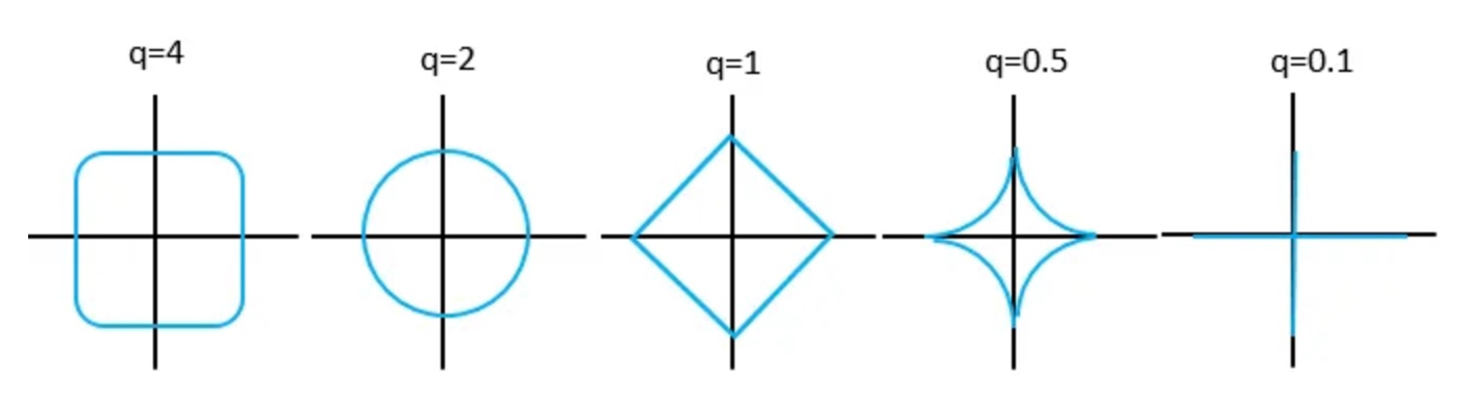
\includegraphics[width=1\linewidth]{Q-values.pdf}
    \caption{\; A geometric visualisation of our penalty term $\lambda$, where $Q=2$ represents Ridge Regression's (see RHS of poster, and $Q=1$ represents LASSO's. These are called constraint regions.}
\end{figure}
As we increase our hyperparameter, {$\lambda$}, our model becomes simpler with fewer variables, while when we decrease {$\lambda$} our model becomes complex with a greater number of parameters. A {$\lambda$} of zero will simply provide us with the OLS. The optimal level of {$\lambda$} is selected through k-fold cross-validation, there is information on this technique in the middle of the poster. LASSO can trace its origins back to a Geophysics paper [1] where the authors used a L1 penalty term on coefficients. However, in 1996 LASSO Regression was formally proposed, and popularised, by Robert Tibshirani [2].}
\begin{figure}
    \centering
    \includegraphics[width=0.65\linewidth]{Bias.Variance.TO1.pdf}
    \caption{\; A visualisation of the ideal balance between bias and variance that LASSO delivers with L1 regularisation.}
\end{figure}
\end{block}

\end{column} % End of the first column

\begin{column}{\sepwid}\end{column} % Empty spacer column

\begin{column}{\twocolwid} % Begin a column which is two columns wide (column 2)

\vspace{-1.25cm}

\begin{block}{LASSO Implementation}

\begin{itemize}
	\item \textbf{Model Motivation} - Predict the Percentage change in price (open/close) for the iShares MSCI Japan ETF (EWJ), traded on the NYSE. With non-overlapping market hours between the NYSE \& TSE, the valuation of this ETF is more complex and so sparked some curiosity. The high dimensionality of our data makes it perfect for the use of LASSO regression, which is suited to deal with large numbers of parameters. The automatic variable selection of LASSO will help reduce over fitting and the penalty terms provide a qualitative interpretation of our parameters contribution to the dependent variable.
	\item \textbf{Execution and Wrangling} - Importing, wrangling, and regularising our data, making it suitable for applying LASSO regression. Sourced from Yahoo Finance, we pulled 84 metrics from 478 trading days to use in training our model, summing to just over \textbf{40,000 total observations}. We used macro indicators such as the US Treasury yield and the US-JPN exchange rate, the financial metrics of the top ten holdings within the ETF, market index price data, and various metrics of volatility and market momentum. Our data was then engineered to ensure it was suitable to work with. This included time lagging in order to account for historic data and time zone differences, splitting into training/testing datasets, and handling any empty entries. After all of this the implementation into our model also required us to include an imputation step to account for n/a values. To carry these tasks out we used functions and frameworks from Sklearn, NumPy and pandas. 
	\item \textbf{Performance and Choice of Hyperparameter} - The below figure shows how our models predictions change as we change our $\lambda$, overall we can see our model is fairly accurate in its prediction.:
 \end{itemize}
    \begin{figure}   
    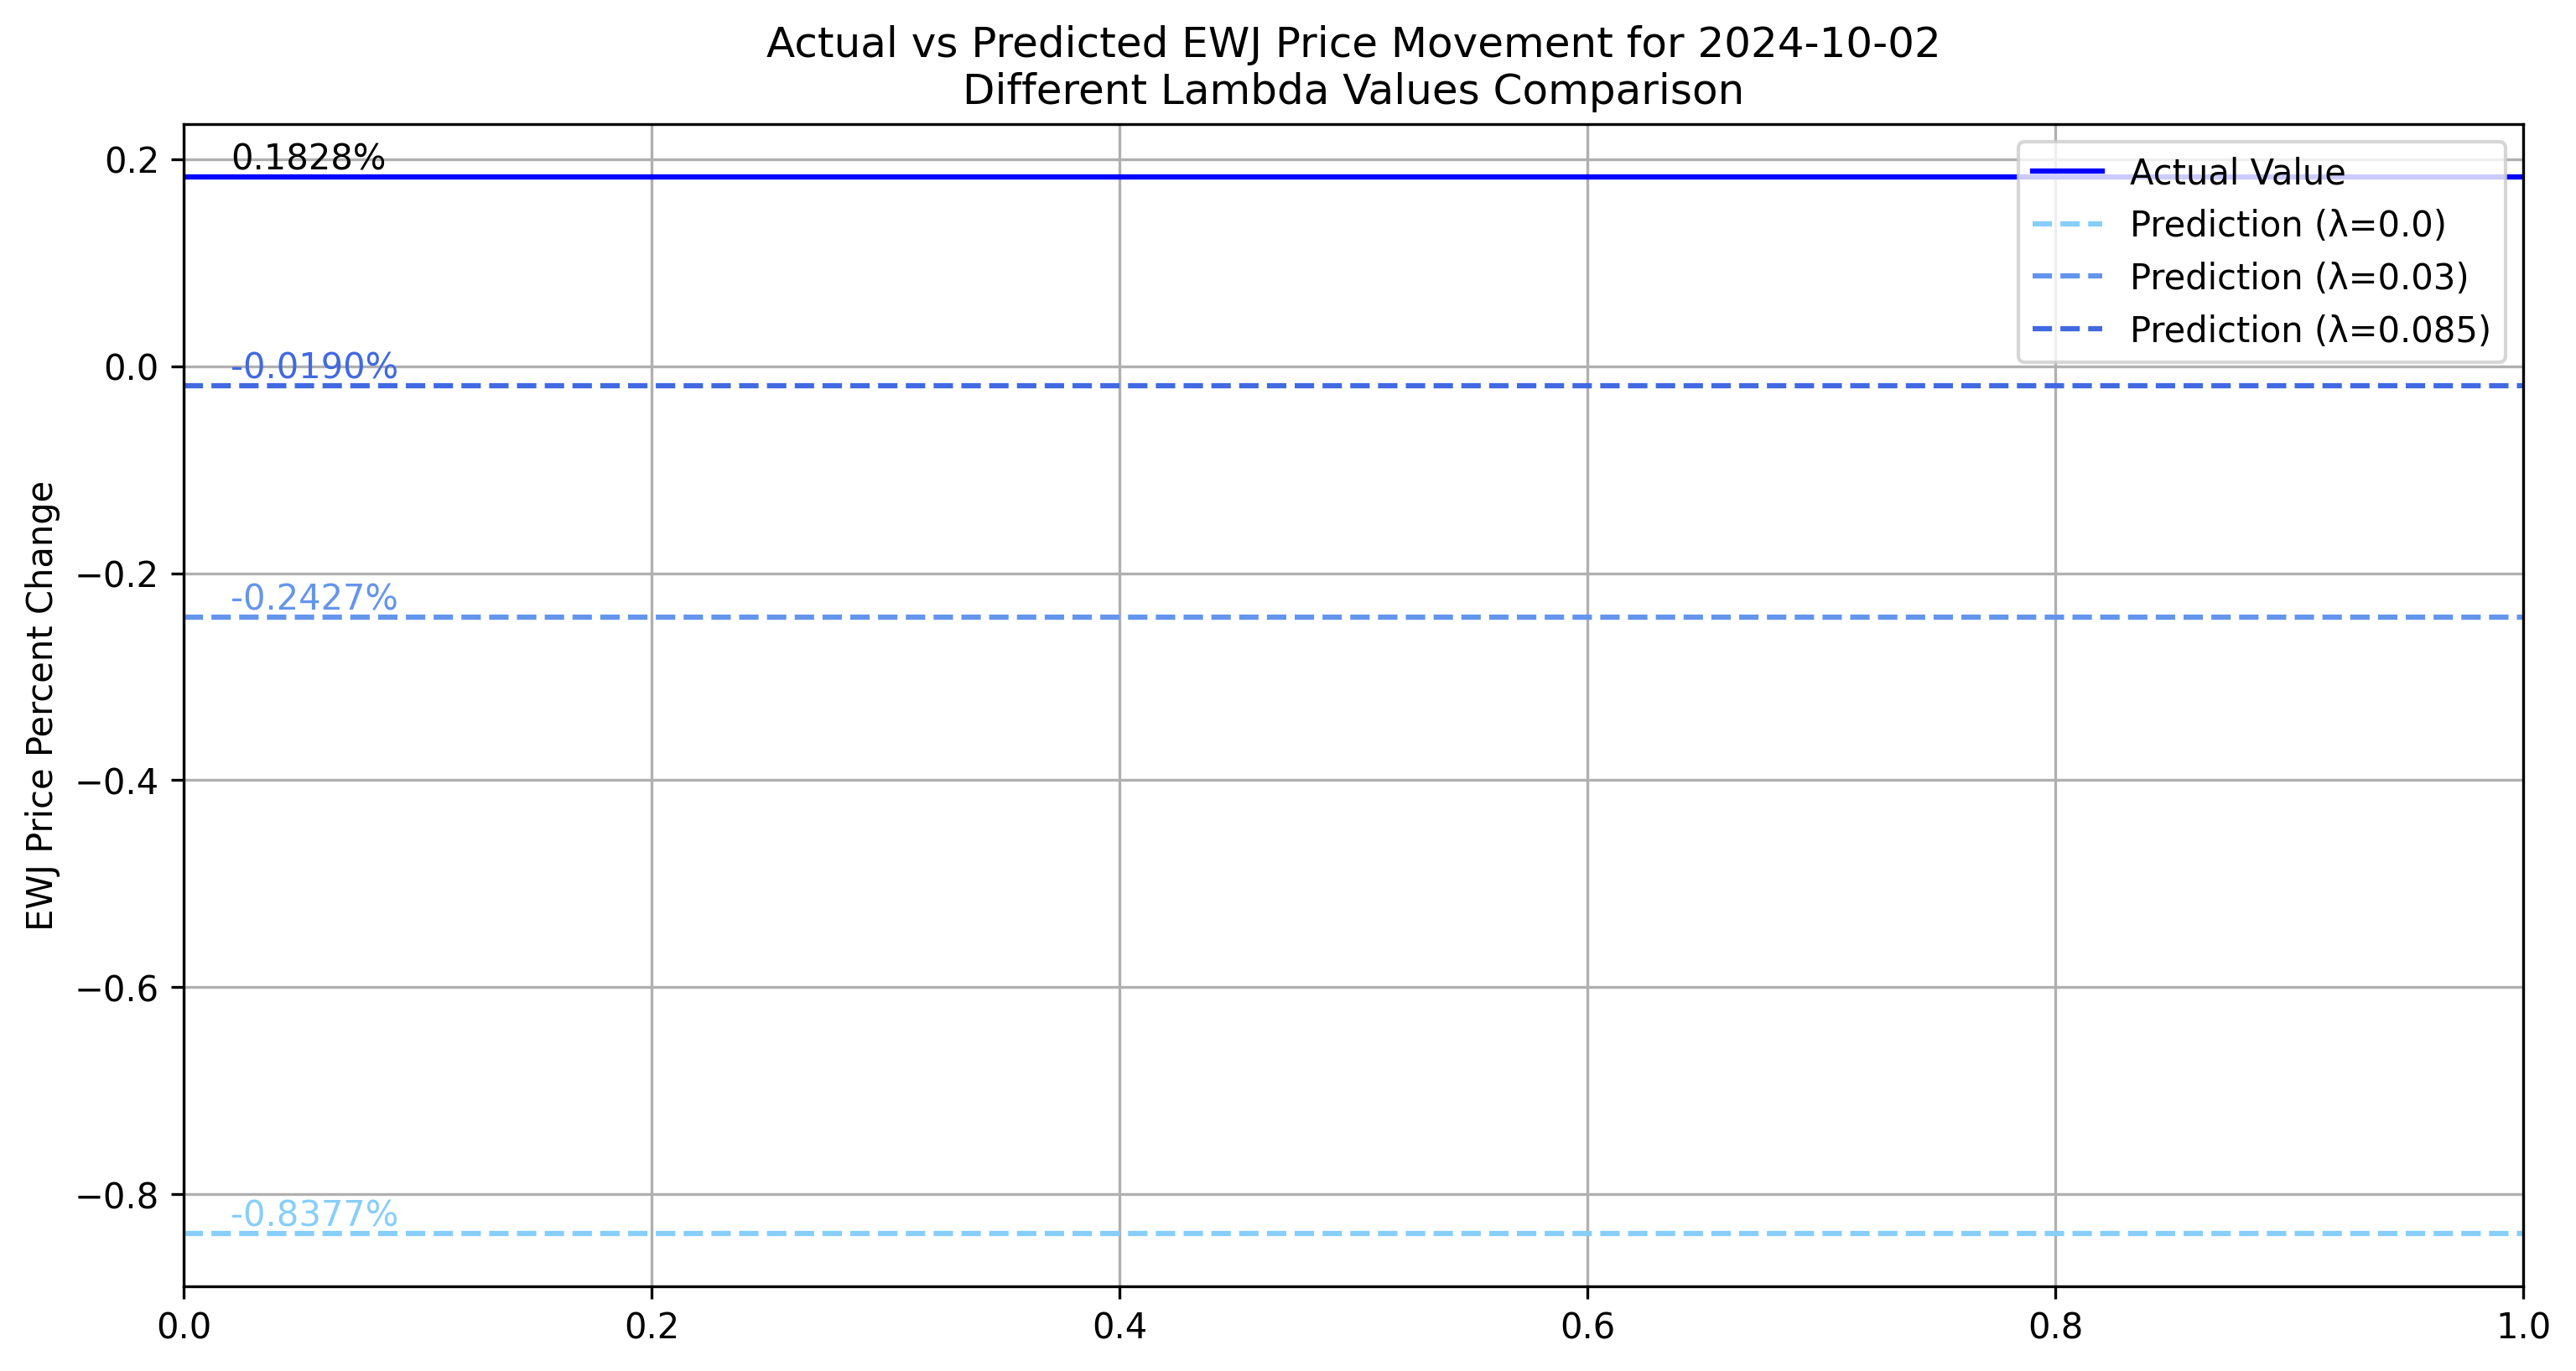
\includegraphics[width=0.4\linewidth]{predictions_comparison_lambda_final.png}
    \caption{Actual vs Predicted ETF Price Movement for 2024-10-02, comparing different choices for $\lambda$.}
\end{figure}
The different choices of $\lambda$ above demonstrates how model accuracy differs with its value. As discussed, increasing $\lambda$ reduces the number of parameters in our model. For $\lambda = 0$ all 84 parameters were retained, leaving us with the $\beta_{OLS}$. At $\lambda = 0.03$, the model is reduced to fourteen parameters and for $\lambda = 0.085$, our model is reduced to a single parameter, the difference between the daily high and low of the Nikkei 225, which is given a negative coefficient. This  suggests that large movements in this index, are correlated with a mean reversion in our ETF, i.e. price falling. To find the optimal value of $\lambda$ one would implement a technique known as K-Fold Cross-Validation, of which information is below.

\end{block} 

    \begin{alertblock}{K-Fold Cross-Validation}
        A resampling procedure that involves randomly shuffling up our dataset and splitting it into k number of equal sized groups, which are then used as training data for the model. The optimal lambda can be found by finding the lambda that produces the best model for each group (lowest MSE) and then finding the average. This process balances the tradeoff between bias and variance, graphed in the bottom left.

    \end{alertblock}
\end{column} % End of the second column

\begin{column}{\sepwid}\end{column} % Empty spacer column

\begin{column}{\onecolwid} % The third column

\vspace{-1.25cm}

\begin{block}{Feature Selection with LASSO Regression compared to Ridge Regression}
    \footnotesize{The most important difference between LASSO and other systems of Regression is that LASSO is able to reduce parameter weights to 0, on the other hand ridge regression is only able to reduce their weight to near zero. This can be shown below in Figure 2, and explained further after that.
    \begin{figure}
        \centering
        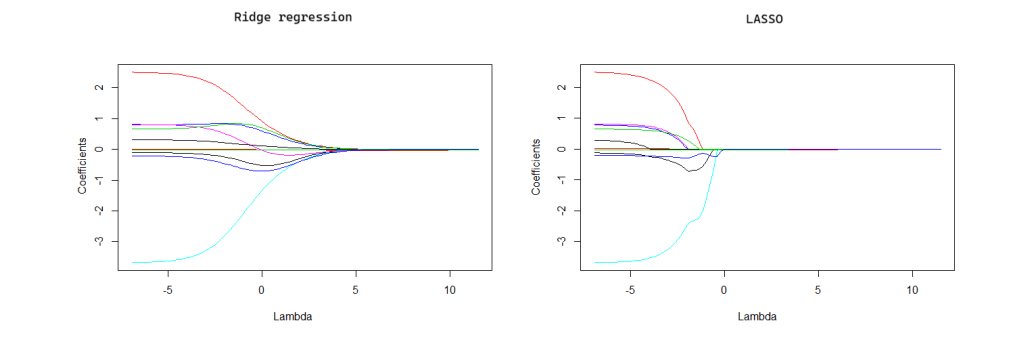
\includegraphics[width=1\linewidth]{Ridge VS LASSO.png}
        \caption{\; A comparison of the behaviour's of biases as $\lambda$ varies, between Ridge Regression and LASSO}
    \end{figure}        
Geometrically, this is due the diamond shape produced by the constraint region of the penalty terms, which has corners on each axis line. The weight coefficients are found where the contours of the RSS first collide with the constraint region, which can be one of the axis lines in LASSO. However, due to the circular shape of the constraint in ridge regression this is impossible, so a weight coefficient can never be 0. Algebraically we can show that for Ridge Regression when we solve for $\Beta$ our expression is asymptotic to $0$ as $\lambda \rightarrow \infty$, however for brevity we leave this out. This means LASSO is much more useful when given a large amount of parameters that are known to be irrelevant to the data.

\begin{figure}
    \centering
    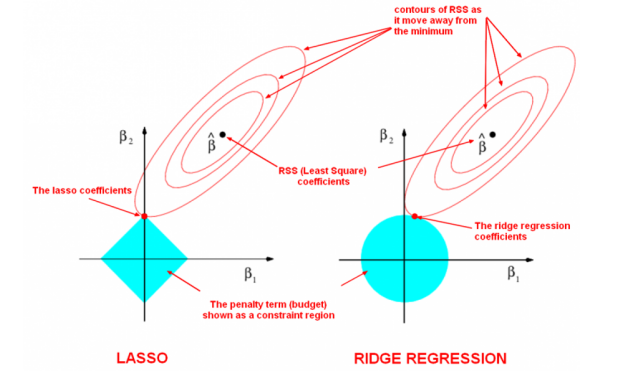
\includegraphics[width=0.75\linewidth]{Geometry.png}
    \caption{\; LASSO vs Ridge Regression geometric RSS and constraint region comparison}
\end{figure}
    However, each have their benefits and drawbacks. LASSO can require considerable computational power, Ridge is extremely useful when we have a set of parameters we know are relevant. LASSO is also less reliable in some instances than Ridge Regression as it has to be optimised iteratively, meaning different optimisation techniques may produce different models.}
\end{block}

\vspace{-0.5cm}

 \begin{block}{References}
\begin{itemize}
\tiny{
\vspace{-0.75cm}
\bibitem[1]{bandLimitedReflection}
Santosa, Fadil, and William W. Symses. 1986. `Linear Inversion of Band-Limited Reflection Seismograms.' \emph{Inverse Problems 2, no. 1 (1986): 1-8.}

\bibitem[2]{robertTibshirani}
Tibshirani, Robert. 1996. `Regression Shrinkage and Selection via the Lasso.' \emph{Journal of the Royal Statistical Society. Series B (Methodological) 58, no. 1 (1996): 267–88}.

\bibitem[3]{ibm}
IBM Resources, https://www.ibm.com/topics/lasso-regression, accessed 20 November 2024.

\bibitem[4]{statisticshowto}
LASSO Regression, https://www.statisticshowto.com/lasso-regression/, accessed 20 November 2024.

\bibitem[5]{hforhr}
Supervised Statistical Learning Using LASSO Regression, https://rforhr.com/lassoregression.html, accessed 23 November 2024.

\bibitem[6]{kitchingroup}
Linear Regression, https://kitchingroup.cheme.cmu.edu/f19-06623/18-linear-regression.html, accessed 23 November 2024.
 }



\end{itemize} 



\end{block}

\end{column} % End of the third column

\end{columns} % End of all the columns in the poster

\end{frame} % End of the enclosing frame

\end{document}
